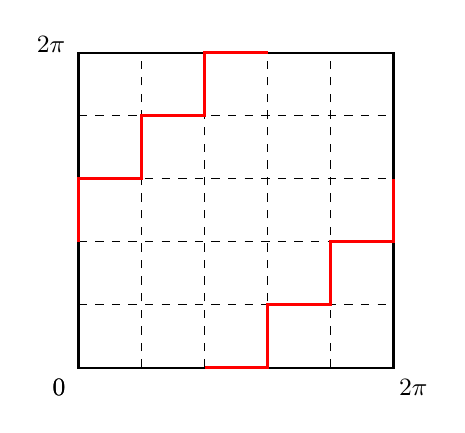
\begin{tikzpicture}[scale=1, every node/.style={font=\small}]
  \def\S{4} % side length of the square

  % --- draw outer square
  \draw[line width=0.9pt] (0,0) rectangle (\S,\S);

  % --- equally spaced dotted lines (4 each direction)
  \foreach \i in {1,2,3,4}{
    % verticals
    \draw[dashed] (\i*\S/5,0) -- (\i*\S/5,\S);
    % horizontals
    \draw[dashed] (0,\i*\S/5) -- (\S,\i*\S/5);
  }

  \draw[red,line width=1.2pt]
    (0,2*\S/5) -- (0,3*\S/5) -- (\S/5,3*\S/5) -- (\S/5,4*\S/5) --
    (2*\S/5,4*\S/5) -- (2*\S/5,5*\S/5) -- (3*\S/5,5*\S/5);
    
  \draw[red,line width=1.2pt]
    (2*\S/5,0) -- (3*\S/5,0) --
    (3*\S/5,\S/5) -- (4*\S/5,\S/5) -- (4*\S/5,2*\S/5) --
    (5*\S/5,2*\S/5) -- (5*\S/5,3*\S/5);

  % --- axis labels
  \node at (-0.25,-0.25) {$0$};
  \node at (\S+0.25,-0.25) {$2\pi$};
  \node at (-0.35,\S+0.1) {$2\pi$};
  \node at (-0.25,-0.25) {$0$};
\end{tikzpicture}